

\section{Optimization in Neural Networks}

A neural network can be seen as a map:
\[
F_{NN}(x) = y
\]

We can define a cost function:
\[
J = \frac{1}{2N} \sum_{i=1}^{N} (\bar{y}_i - y_i)^2
\]

Inside $F_{NN}$, we have nodes that represent weights $w$ and biases $b$, chosen to minimize $J$:
\[
(w, b) = \argmin J
\]

The objective in machine learning is not only to find $w$ and $b$ to build the function $F_{NN}$ minimizing $J$, but also to create $F_{NN}$ capable of making predictions (train set $\neq$ test set).

In the optimization context, we want to get closer to the minimum $J$ without overfitting (i.e., the model should understand the underlying pattern of the data, not just memorize it).

The gradient method, particularly its variant Stochastic Gradient Descent (SGD), is the most used method in machine learning. It is simple and robust (can be implemented with non-convex functions, though theoretical guarantees are for convex ones).

Let's recall its application to linear systems:
\[
Ax = b
\]
with solution $x^*$, where $A \in \mathbb{R}^{n \times n}$ is a symmetric positive definite matrix.

We define the functional:
\[
J(x) = \frac{1}{2} x^T A x - x^T b
\]

To find the minimum:
\[
\begin{aligned}
\nabla J(x) &= Ax - b = 0 \\
&\Rightarrow Ax^* = b
\end{aligned}
\]

\subsubsection*{Algorithm}
Given an initial guess $x^{(0)}$:

For $k = 0, 1, \ldots$:
\begin{enumerate}
    \item $p^{(k)} = -\nabla J(x^{(k)}) = r^{(k)}$
    \item $x^{(k+1)} = x^{(k)} + \alpha_k p^{(k)}$
\end{enumerate}

where $\alpha_k$ is the step length, chosen to minimize $J(x^{(k)} + \alpha p^{(k)})$.

Stopping criteria: $\|r^{(k)}\| \leq \varepsilon$ or $\|x^{(k+1)} - x^{(k)}\| < \varepsilon$

\subsubsection*{Step Length Calculation}
Suppose $x^{(k)}$ and $p^{(k)}$ are given:
\[
\begin{aligned}
J(x^{(k)} + \alpha p^{(k)}) &= \frac{1}{2}(x^{(k)} + \alpha p^{(k)})^T A (x^{(k)} + \alpha p^{(k)}) - (x^{(k)} + \alpha p^{(k)})^T b \\
&= \frac{1}{2}\alpha^2 (p^{(k)})^T A p^{(k)} + \alpha (p^{(k)})^T A x^{(k)} - \alpha (p^{(k)})^T b + \text{constants}
\end{aligned}
\]

Setting the derivative to zero:
\[
\begin{aligned}
\nabla J = 0 &= (p^{(k)})^T A x^{(k)} + \alpha (p^{(k)})^T A p^{(k)} - (p^{(k)})^T b \\
\Rightarrow \alpha &= \frac{(p^{(k)})^T (b -A x^{(k)} )}{(p^{(k)})^T A p^{(k)}} = \frac{(p^{(k)})^T r^{(k)}}{(p^{(k)})^T A p^{(k)}}
\end{aligned}
\]

Define the error, in the energy norm of the matrix A:
\[
e = \frac{1}{2}(x - x^*)^T A (x - x^*)
\]

Error bound:
\[
e(x^{(k)}) \leq \left(\frac{\lambda_{\max} - \lambda_{\min}}{\lambda_{\max} + \lambda_{\min}}\right)^{2k} e(x^{(0)})
\]

where $\lambda_{\max}$ and $\lambda_{\min}$ are the maximum and minimum eigenvalues of $A$.

\subsection*{General Convex Optimization}
Now let $J: \mathbb{R}^d \to \mathbb{R}$ be convex and differentiable, with a global minimum $x^*$. The aim is to find an approximation $\tilde{x}$ of $x^*$ such that:
\[
J(\tilde{x}) - J(x^*) < \varepsilon
\]

\subsubsection*{Algorithm}
Generate a sequence $x^{(0)}, x^{(1)}, \ldots$ using the rule:
\[
x^{(k+1)} = x^{(k)} + v^{(k)}
\]

To guarantee $J(x^{(k+1)}) < J(x^{(k)})$:
\[
\begin{aligned}
J(\mathbf{x}^{(k)} + \mathbf{v}^{(k)}) \approx J(\mathbf{x}^{(k)}) + \nabla J(\mathbf{x}^{(k)})^T\mathbf{v}^{(k)} + \mathcal{O}(\|\mathbf{v}^{(k)}\|^2)
\end{aligned}
\]

Therefore, we can move in the direction of maximum descent by following this rule:

\[
\begin{aligned}
v^{(k)} = -\alpha\nabla J(x^{(k)}), \quad \alpha > 0 \\
x^{(k+1)} = x^{(k)} - \gamma \nabla J(x^{(k)})\\
\end{aligned}
\]

where $\gamma$ is the learning rate.


Remember that:
\begin{itemize}
    \item $\gamma$ can be fixed or can depend on $k$
    \item Choice of $\gamma$ is crucial:
    \begin{itemize}
        \item If too small: very slow procedure
        \item If too large: overshooting (oscillating behavior)
    \end{itemize}
\end{itemize}

\subsection*{Convexity Criterion}
For $J(x), x \in \mathbb{R}^d$, if the domain of $J$ is convex, then $J$ is convex if and only if:
\[
J(y) \geq J(x) + \nabla J(x)^T(y-x) \quad \forall x, y \in \text{dom}(J)
\]
This means the graph of function $J$ lies above the tangent hyperplane to $J$ in $x$.

A convex function has the property of monotonicity of the gradient.\\ \\
\textbf{Monotonicity of the Gradient} \\
A function's gradient \( \nabla f \) is said to be monotone if for all \( x, y \in \mathbb{R}^n \),
\[
(\nabla f(y) - \nabla f(x))^\top (y - x) \geq 0
\]

\subsection{Convergence Analysis}
Let's analyze the convergence of the method. If $J$ is convex, then:
\[
J(x^{(k)}) - J(x^*) \leq \underbrace{\nabla J(x^{(k)})^T}_{e^{(k)}}(x^{(k)} - x^*)
\]

For the iteration that defines the method:
\[
\begin{aligned}
e^{(k)} &= \frac{x^{(k)} - x^{(k+1)}}{\gamma} \\
\Rightarrow (e^{(k)})^T(x^{(k)} - x^*) &= \frac{1}{\gamma}(x^{(k)} - x^{(k+1)})^T(x^{(k)} - x^*)
\end{aligned}
\]

Now I will derive an easy identity:
\begin{enumerate}
\item \(\|v - w\|^2 = (v - w)^T (v - w)\)\\
\item \(\|v - w\|^2 = v^T v - 2v^T w + w^T w\)\\
\item \(\|v - w\|^2 = \|v\|^2 - 2v^T w + \|w\|^2\)\\
\item \(2v^T w = \|v\|^2 + \|w\|^2 - \|v - w\|^2\)\\
\end{enumerate}
Using the identity $2v^Tw = \|v\|^2 + \|w\|^2 - \|v-w\|^2$, we get:
\[
\begin{aligned}
(e^{(k)})^T(x^{(k)} - x^*) &= \frac{1}{2\gamma}[\|x^{(k)} - x^{(k+1)}\|^2 + \|x^{(k)} - x^*\|^2 - \|x^{(k+1)} - x^*\|^2] \\
&= \frac{1}{2\gamma}[\gamma^2\|e^{(k)}\|^2 + \|x^{(k)} - x^*\|^2 - \|x^{(k+1)} - x^*\|^2] \\
&= \frac{\gamma}{2}\|e^{(k)}\|^2 + \frac{1}{2\gamma}[\|x^{(k)} - x^*\|^2 - \frac{1}{2}\|x^{(k+1)} - x^*\|^2]
\end{aligned}
\]

Summing over iterations:
\[
\begin{aligned}
\sum_{k=0}^{T-1}(e^{(k)})^T(x^{(k)} - x^*) &= \frac{\gamma}{2}\sum_{k=0}^{T-1}\|e^{(k)}\|^2 + \frac{1}{2\gamma}[\|x^{(0)} - x^*\|^2 -\frac{1}{2\gamma} \|x^{(T)} - x^*\|^2] \\
&\leq \frac{\gamma}{2}\sum_{k=0}^{T-1}\|e^{(k)}\|^2 + \frac{1}{2\gamma}\|x^{(0)} - x^*\|^2
\end{aligned}
\]

Therefore:
\[
\sum_{k=0}^{T-1}(J(x^{(k)}) - J(x^*)) \leq \frac{\gamma}{2}\sum_{k=0}^{T-1}\|e^{(k)}\|^2 + \frac{1}{2\gamma}\|x^{(0)} - x^*\|^2
\]

\subsection{Convergence Theorem for Lipschitz Convex Functions}
Let $J: \mathbb{R}^d \to \mathbb{R}$ be convex and differentiable, and also:
\begin{itemize}
    \item $\|x^{(0)} - x^*\| \leq R$
    \item $\|\nabla J(x)\| \leq B \quad \forall x$
\end{itemize}

\begin{theorem}
If we choose $\gamma := \frac{R}{B\sqrt{T}}$, then:
\[
\frac{1}{T}\sum_{k=0}^{T-1}(J(x^{(k)}) - J(x^*)) \leq \frac{RB}{\sqrt{T}}
\]
\end{theorem}

To achieve a certain tolerance $\varepsilon$:
\[
\begin{aligned}
\frac{RB}{\sqrt{T}} &< \varepsilon \\
T &\geq \frac{R^2B^2}{\varepsilon^2}
\end{aligned}
\]

Note: There's no dependence on $d$! The number of iterations is $O(1/\varepsilon^2)$.

The previous relation can be bounded:
\[
\sum_{k=0}^{T-1}(J(x^{(k)}) - J(x^*)) \leq \underbrace{\frac{\gamma}{2}B^2T + \frac{R^2}{2\gamma}}_{q(\gamma)}
\]

We want to find $\gamma$ to minimize $q$. Set $q'(\gamma) = 0$:
\[
\begin{aligned}
\frac{1}{2}B^2T - \frac{R^2}{2\gamma^2} &= 0 \\
\gamma &= \frac{R}{B\sqrt{T}}
\end{aligned}
\]

\subsection*{Proof of Convergence Theorem}
\begin{proof}
The previous relation can be bounded:
\[
\sum_{k=0}^{T-1}(J(x^{(k)}) - J(x^*)) \leq \underbrace{\frac{\gamma}{2}B^2T + \frac{R^2}{2\gamma}}_{q(\gamma)}
\]

We want to find $\gamma$ to minimize $q$. Set $q'(\gamma) = 0$:
\[
\begin{aligned}
\frac{1}{2}B^2T - \frac{R^2}{2\gamma^2} &= 0 \\
\gamma &= \frac{R}{B\sqrt{T}}
\end{aligned}
\]

Therefore:
\[
q\left(\gamma = \frac{R}{B\sqrt{T}}\right) = RB\sqrt{T}
\]
\end{proof}

\subsection*{Equivalence of Smoothness and Convexity}


Let $\text{dom}(J)$ be open and convex, and $J: \text{dom}(J) \to \mathbb{R}$ be differentiable. Let $L \in \mathbb{R}^+$. \\ 
$J$ is said to be L-smooth (or smooth with parameter L) if it satisfies the following smoothness inequality for all $x, y \in \text{dom}(J)$:
$$J(y) \leq J(x) + \nabla J(x)^T(y-x) + \frac{L}{2}\|y-x\|^2$$

\begin{lemma}
Let $\text{dom}(J)$ be open and convex, and $J: \text{dom}(J) \to \mathbb{R}$ be differentiable.
Let $L \in \mathbb{R}^+$. The following statements are equivalent:
\begin{enumerate}
    \item $J$ is smooth with parameter $L$
    \item The function $h(x) = \frac{L}{2}x^Tx - J(x)$ is convex over $\text{dom}(h) := \text{dom}(J)$
\end{enumerate}
\end{lemma}


\paragraph{Example 1: $L = 0$}
When $L = 0$, smoothness implies:
\[
J(y) = J(x) + \nabla J(x)^T(y-x)
\]

\paragraph{Example 2: $J(x) = x^2$}
This function is not globally Lipschitz continuous, but it is smooth (has a Lipschitz continuous gradient).

Let's expand $J(y)$ around $x$:
\begin{align*}
J(y) &= y^2 \\
&= (x + (y-x))^2 \\
&= x^2 + 2x(y-x) + (y-x)^2 \\
&= J(x) + \nabla J(x)^T(y-x) + (y-x)^2
\end{align*}

Explanation of the expansion:
\begin{itemize}
    \item $J(x) = x^2$ is our original function at point $x$
    \item $\nabla J(x) = 2x$, so $\nabla J(x)^T(y-x) = 2x(y-x)$
    \item The term $(y-x)^2$ is the remainder
\end{itemize}

This expansion matches the form of the smoothness condition:
\[
J(y) \leq J(x) + \nabla J(x)^T(y-x) + \frac{L}{2}(y-x)^2
\]

In this case, the inequality is an equality with $\frac{L}{2} = 1$, so $L = 2$.

To verify smoothness, we check the gradient condition:
\[
|\nabla J(y) - \nabla J(x)| = |2y - 2x| = 2|y-x| \leq L|y-x|
\]
which is satisfied with $L = 2$.

Therefore, $J(x) = x^2$ is a smooth function with parameter $L = 2$. 
This example illustrates that a function can be smooth without being globally Lipschitz continuous.
\paragraph{Example 3: Quadratic Function}
Consider $J(x) = x^TQx + b^Tx + c$, where:
\begin{itemize}
    \item $Q \in \mathbb{R}^{d \times d}$ is symmetric
    \item $b \in \mathbb{R}^d$
    \item $c \in \mathbb{R}$
\end{itemize}
This function is smooth with $L = 2\|Q\|_2$, where $\|Q\|_2$ is the spectral norm of $Q$.

\textbf{Note:} Subquadratic functions are not necessarily smooth.\subsection*{Equivalence Lemma for Smooth Functions}
\begin{lemma}
Let $J: \mathbb{R}^d \to \mathbb{R}$ be convex and differentiable.
The following statements are equivalent:
\begin{itemize}
    \item $J$ is smooth with parameter $L$
    \item $\|\nabla J(x) - \nabla J(y)\| \leq L\|y-x\| \quad \forall x, y \in \mathbb{R}^d$ (Lipschitz continuity of gradient)
\end{itemize}
\end{lemma}

\subsection{Decreasing Condition Lemma}
\begin{lemma}[Decreasing Condition]
Let $J: \mathbb{R}^d \to \mathbb{R}$ be differentiable and smooth with parameter $L$. With $\gamma := \frac{1}{L}$, the Gradient Descent satisfies:
\[
J(x^{(k+1)}) \leq J(x^{(k)}) - \frac{1}{2L}\|\nabla J(x^{(k)})\|^2 \quad k \geq 0
\]
\end{lemma}

\begin{proof}
The Gradient Descent update is given by:
\[
x^{(k+1)} = x^{(k)} - \frac{1}{L}\nabla J(x^{(k)})
\]

By the smoothness property:
\begin{align*}
J(x^{(k+1)}) &\leq J(x^{(k)}) + (\nabla J(x^{(k)}))^T(x^{(k+1)} - x^{(k)}) + \frac{L}{2}\|x^{(k+1)} - x^{(k)}\|^2 \\
&= J(x^{(k)}) - (\nabla J(x^{(k)}))^T\frac{1}{L}\nabla J(x^{(k)}) + \frac{L}{2}\|\frac{1}{L}\nabla J(x^{(k)})\|^2 \\
&= J(x^{(k)}) - \frac{1}{2L}\|\nabla J(x^{(k)})\|^2
\end{align*}
\end{proof}

\subsection{Convergence Theorem for Smooth Functions}
\begin{theorem}
Let $J: \mathbb{R}^d \to \mathbb{R}$ be differentiable and smooth with parameter $L$.
Choosing $\gamma := \frac{1}{L}$, then for Gradient Descent you have:
\[
J(x^{(T)}) - J(x^*) \leq \frac{L}{2T}\|x^{(0)} - x^*\|^2, \quad \quad  T > 0
\]
where $x^*$ is the optimal point.
\end{theorem}
\\ \\
\begin{proof}
From the decreasing condition lemma, and the usual telescopic sum formula:
\[
\frac{1}{2L}\sum_{k=0}^{T-1}\|\nabla J(x^{(k)})\|^2 \leq \sum_{k=0}^{T-1}(J(x^{(k)}) - J(x^{(k+1)})) = J(x^{(0)}) - J(x^{(T)})
\]
Remembering that:
$$
|| e^{k} ||^2 = || \nabla J(x^{(k)}) ||^2
$$
We know that:
\[
\sum_{k=0}^{T-1}(J(x^{(k)}) - J(x^*)) \leq \frac{\gamma}{2}\sum_{k=0}^{T-1}\|e^{(k)}\|^2 + \frac{1}{2\gamma}\|x^{(0)} - x^*\|^2
\]

For $\gamma = \frac{1}{L}$:
\begin{align*}
\sum_{k=0}^{T-1}(J(x^{(k)}) - J(x^*)) &\leq \frac{1}{2L}\sum_{k=0}^{T-1}\|e^{(k)}\|^2 + \frac{L}{2}\|x^{(0)} - x^*\|^2 \\
&\leq J(x^{(0)}) - J(x^{(T)}) + \frac{L}{2}\|x^{(0)} - x^*\|^2 \\
\Rightarrow \sum_{k=1}^{T}(J(x^{(k)}) - J(x^*)) &\leq \frac{L}{2}\|x^{(0)} - x^*\|^2
\end{align*}

By the decreasing condition lemma, $J(x^{(k+1)}) \leq J(x^{(k)}) \quad \forall \ 0 \leq k \leq T$, so:
\[
J(x^{(T)}) - J(x^*) \leq \frac{1}{T}\sum_{k=1}^{T}(J(x^{(k)}) - J(x^*)) \leq \frac{L}{2T}\|x^{(0)} - x^*\|^2
\]
\end{proof}


\subsection*{Convergence results for Gradient Descent}
\begin{itemize}
    \item Lipschitz-convex functions: $O\left(\dfrac{1}{\epsilon^2}\right)$
    \item Smooth functions: $O\left(\dfrac{1}{\epsilon}\right)$
    \item Smooth and strongy convex functions: $O\left(\dfrac{1}{\log(\epsilon)}\right)$
    \item Accelerated gradient descent: $O\left(\dfrac{1}{\sqrt{\epsilon}}\right)$
\end{itemize}


\section{Accelerated Gradient Descent}
Aim: minimizing convex function $f: \mathbb{R}^d \to \mathbb{R}$ (with gradient $\nabla f$). "First order method" because it only uses the function and its gradient. What is the best first order method?\\
Nemirovski and Yudin (1979): every first order method needs in the worst case $O\left(\dfrac{1}{\sqrt{\epsilon}}\right)$ steps. \\
Nesterov (1983): accelerated gradient descent (AGD). Let $f: \mathbb{R}^d \to \mathbb{R}$ convex, differentiable and smooth with parameter $L$. ADG reads:
\begin{itemize}
    \item choose $\underline{z}^{(0)} = \underline{y}^{(0)} = \underline{x}^{(0)}$
    \item for $k \geq 0$ set:
    \begin{itemize}
        \item $\underline{y}^{(k+1)} = \underline{x}^{(k)} - \dfrac{1}{L} \nabla f(\underline{x}^{(k)})$ \hspace{2cm} Normal step
        \item $\underline{z}^{(k+1)} = \underline{z}^{(k)} - \dfrac{k+1}{2L} \nabla f (\underline{x}^{(k)})$ \hspace{2cm} Aggressive step
        \item $\underline{x}^{(k+1)} = \dfrac{k+1}{k+3} \underline{y}^{(k+1)} + \dfrac{2}{k+3} \underline{z}^{(k+1)}$ \hspace{2cm} Average 
    \end{itemize}
\end{itemize}

\textbf{Theorem of convergence of AGD}: lef $f: \mathbb{R}^d \to \mathbb{R}$ convex, differentiable with a global minimum $\underline{x}^*$ and smooth with parameter $L$. AGD yields:
\[
f(\underline{y}^{(N)}) - f(\underline{x}^*) \leq \dfrac{2L \Vert \underline{z}^{(0)} - \underline{x}^* \Vert^2}{N(N+1)}  \hspace{1cm} N > 0   
\]
\textbf{Definition of smooth and strongly convex functions}: Let $f: \text{dom}(f) \to \mathbb{R}$ be a convex and differentiable function, $X \subseteq \text{dom}(f)$ convex and $\mu \in \mathbb{R}^+$. Function $f$ is called strongly convex with parameter $\mu$ over $X$ if:
\[
f(\underline{y}) \geq f(\underline{x}) + \nabla f(\underline{x})^T (\underline{y} - \underline{x}) + \dfrac{\mu}{2} \Vert \underline{y} - \underline{x} \Vert^2 \hspace{1cm} \forall \underline{x}, \underline{y} \in X    
\] 
Remark
\begin{itemize}
    \item \textbf{smoothness}: $\forall \underline{x} \in X$ the graph of $f$ is below a not-too-steep tangent paraboloid.
    \item \textbf{Strongly-convex}: $\forall \underline{x} \in X$ the graph of $f$ is above a not-too-flat tangent paraboloid.\\ 
\end{itemize}

Theorem of convergence: strongly convex case: let $f: \mathbb{R}^d \to \mathbb{R}$ be a convex, differentiable. Suppose that $f$ is smooth with parameter $L$ and strongly convex with parameter $\mu$ > 0. Choosing:
\[
    \nu = \dfrac{1}{L}    
\]
Gradient Descent with arbitrary initial point $\underline{x}^{(0)}$ satisfies:
\begin{enumerate}
    \item Squared distances to $\underline{x}^*$ are geometrically decreasing: $\Vert \underline{x}^{(k+1)} - \underline{x}^* \Vert^2 \leq \left(1-\dfrac{\mu}{L}\right)\Vert \underline{x}^{(k)} - \underline{x}^* \Vert^2$ \hspace{1cm} $k \geq 0$
    \item Absolute error after N iterations is exponentially small in N: $f(\underline{x}^{(N)}) - f(\underline{x}^*) \leq \dfrac{L}{2}\left(1-\dfrac{\mu}{L}\right)^N \Vert \underline{x}^{(0)} - \underline{x}^* \Vert^2$ \hspace{1cm} $N > 0$
\end{enumerate}
Remember: recalling that $\ln(1+x)\leq x$ we have:
\[
    N \geq \dfrac{L}{\mu} \ln\left(\dfrac{R^2 L}{2\epsilon}\right)    
\]

\subsection*{Derivation of last inequality}

Let $R^2 = \|x^{(0)} - x^*\|^2$. Then:

\[
\frac{LR^2}{2}\left(1 - \frac{\mu}{L}\right)^N \leq \varepsilon
\]

Taking logarithms of both sides:

\[
\ln\left(\frac{LR^2}{2}\right) + N\ln\left(1 - \frac{\mu}{L}\right) \leq \ln(\varepsilon)
\]

Rearranging:

\[
N\ln\left(1 - \frac{\mu}{L}\right) \leq \ln(\varepsilon) - \ln\left(\frac{LR^2}{2}\right)
\]

Dividing both sides by $\ln\left(1 - \frac{\mu}{L}\right)\ln\left(1 - \frac{\mu}{L}\right)$ (note that this is negative, so the inequality flips):

\[
N \geq \frac{\ln\left(\frac{2\varepsilon}{LR^2}\right)}{\ln\left(\frac{L-\mu}{L}\right)}
\]

Now, we can use the inequality $\ln(1+x) \leq x\ln(1+x) \leq x for x > -1x > -1. Let x = -\frac{\mu}{L}x = -\frac{\mu}{L}.$ Then:

\[
\ln\left(1 - \frac{\mu}{L}\right) \leq -\frac{\mu}{L}
\]

Therefore:

\[
N \geq \frac{\ln\left(\frac{2\varepsilon}{LR^2}\right)}{-\frac{\mu}{L}} = \frac{L}{\mu}\ln\left(\frac{LR^2}{2\varepsilon}\right)
\]



\newpage
\section{Stochastic Gradient Descent (SGD)}

In machine learning, cost functions are often written as a finite sum:
\[
J(x) = \frac{1}{N}\sum_{i=1}^N J_i(x)
\]
Since in application we have to compute the gradient of $N$ cost functions to calculate $\nabla J$, the idea is to pick randomly an integer $i(K) \in\{1,2, \ldots, N\}$ at each iteration $K$ and use the following iteration rule.
The SGD update rule is:
\[
x^{(k+1)} = x^{(k)} - \gamma_k \nabla J_{i(k)}(x^{(k)})
\]
where $i(k)$ is randomly chosen from $\{1, 2, \ldots, N\}$ at each iteration.

While in Gradient Descent (GD) the cost function decreases at each iteration, the stochastic version is not monotone (but still converges). It typically consists of two phases:
\begin{enumerate}
    \item It converges quickly to a neighborhood of the solution
    \item It bounces around this neighborhood
\end{enumerate}

\subsection*{Example Cost Function}

Consider the cost function:

\[J(x) = \frac{1}{2} \sum_{i=1}^{N} (a_i x - b_i)^2 \quad a_i, b_i \in \mathbb{R}\]

The gradient and optimal solution are:

\begin{align*}
    \nabla J(x) &= \sum_{i=1}^{N} a_i(a_i x - b_i) = 0 \\
    x^* &= \frac{\sum_{i=1}^{N} a_i b_i}{\sum_{i=1}^{N} a_i^2}
\end{align*}

For individual terms:

\begin{align*}
    \bar{J}_i(x) &= \frac{1}{2}(a_i x - b_i)^2 \quad \text{(parabolas)} \\
    \nabla J_i(x) &= a_i(a_i x - b_i) \\
    x_i^* &= \frac{b_i}{a_i}
\end{align*}

\subsection*{Region of Confusion}

Define the region of confusion as:

\[R := [\min_i x_i^*, \max_i x_i^*] \quad \text{where } x^* \in R\]

The area outside $ \Omega \setminus R$ is called the "far out zone." If $x$ is outside of $R$, then $\nabla J_i(x)$ has the same sign as $\nabla J(x)$.
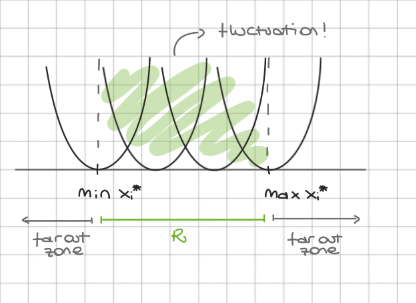
\includegraphics[]{namltexnotes/images/Screenshot 2024-06-26 110851.png}
\\There are two strategies for choosing samples at each iteration:

\begin{enumerate}
    \item Random sampling with replacement
    \item Random sampling without replacement
\end{enumerate}


The second option is better for hardware efficiency, while the first is theoretically better for convergence.

\subsection*{Mini-Batch Approach}

The mini-batch approach uses more than one sample to compute $\nabla J$:

\[\varepsilon_k = \frac{1}{|I_k|} \sum_{i_k \in I_k} \nabla J_{i_k}(x^{(k)}) \quad I_k \subset I\]

where:
\begin{itemize}
    \item If $|I_k| = 1$, we have stochastic gradient descent
    \item If $I_k = I$, we have batch gradient descent
\end{itemize}

This strategy reduces the noise (variance) introduced by using only one sample.
Unlike stochastic gradient descent (SGD) which uses just one sample to compute the gradient, the mini-batch approach uses multiple samples (equal to the batch size) to compute $\nabla J$ (the gradient of the cost function).

The mini-batch gradient estimate is given by:

\begin{equation}
    \varepsilon_{k} = \frac{1}{|I_{k}|} \sum_{i_{k} \in I_{k}} \nabla J_{i_{k}}(x^{(k)})
\end{equation}

Where:
\begin{itemize}
    \item $I_{k}$ is a subset of the full dataset $I$
    \item $|I_{k}|$ is the size of the mini-batch
\end{itemize}

Special cases:
\begin{itemize}
    \item When $|I_{k}| = 1$, you have stochastic gradient descent (SGD)
    \item When $I_{k} = I$ (i.e., the full dataset), you have batch gradient descent
\end{itemize}

Advantages of mini-batch gradient descent:
\begin{itemize}
    \item \textbf{Noise Reduction}: Mini-batch reduces the noise (variance) introduced by using only one sample, as in SGD.
    \item \textbf{Parallelizability}: Mini-batch allows for efficient parallelization of computations, which is particularly beneficial when using GPUs or multi-core CPUs. This leads to faster training times and better hardware utilization.
    \item \textbf{Balance}: It offers a good balance between the frequent updates of SGD and the stability of batch gradient descent.
\end{itemize}

In neural networks, it's generally better not to use very large mini-batches because:
\begin{itemize}
    \item Large mini-batches can create overfitting problems.
    \item They may shrink the region of convergence.
    \item They can potentially reduce the model's generalization ability.
\end{itemize}

The optimal mini-batch size often depends on the specific problem and available computational resources.



\subsection{Equivalent Statements}



The following statements are equivalent:

\begin{enumerate}[a)]
    \item $J(y) \geq J(x) + (\nabla J(x))^T(y-x) + \frac{\mu}{2}\|x-y\|^2$ (strongly convex)
    \item $K(x) = J(x) - \frac{\mu}{2}\|x\|^2$ is convex
    \item $(\nabla J(y) - \nabla J(x))^T(y-x) \geq \mu\|x-y\|^2$
    \item $\frac{1}{2}\|\nabla J(x)\|^2 \geq \mu(J(x) - J(x^*))$ (Polyak-Łojasiewicz (PL) condition)
\end{enumerate}

\subsubsection*{Proof}

\paragraph{(b) $\iff$ (a)}

\begin{align*}
    K(y) & \geq K(x) + \nabla K^\top(x)(y-x) && \text{[given inequality]} \\[10pt]
    \left(J(y) - \frac{\mu}{2}\|y\|^2\right) & \geq \left(J(x) - \frac{\mu}{2}\|x\|^2\right) + \nabla K^\top(x)(y-x) && \text{[substitute $K(y)$ and $K(x)$]} \\[10pt]
    J(y) & \geq J(x) + \frac{\mu}{2}(\|y\|^2 - \|x\|^2) + \left(\nabla J(x) - \mu x^\top\right)(y-x) && \text{[rearrange terms]} \\[10pt]
    & = J(x) + \frac{\mu}{2}(\|y\|^2 - \|x\|^2) + \nabla J^\top(x)(y-x) - \mu x^\top(y-x) && \text{[expand $\nabla K^\top(x)$]} \\[10pt]
    & = J(x) + \nabla J^\top(x)(y-x) + \frac{\mu}{2}(\|y\|^2 - \|x\|^2) - \mu x^\top(y-x) && \text{[group gradient terms]} \\[10pt]
    & = J(x) + \nabla J^\top(x)(y-x) + \frac{\mu}{2}(2x^\top(y-x) + \|y-x\|^2) - \mu x^\top(y-x) && \text{[vector identity]} \\[10pt]
    & = J(x) + \nabla J^\top(x)(y-x) + \mu x^\top(y-x) + \frac{\mu}{2}\|y-x\|^2 - \mu x^\top(y-x) && \text{[distribute $\frac{\mu}{2}$]} \\[10pt]
    & = J(x) + \nabla J^\top(x)(y-x) + \frac{\mu}{2}\|y-x\|^2 && \text{[simplify, cancel terms]}
\end{align*}



\paragraph{(b) ⟹\implies (c)}

By the monotonicity of the gradient:
\begin{align*}
    (\nabla K(y) - \nabla K(x))^\top(y-x) &\geq 0 \quad \forall x, y \\
    \left[\nabla\left(J(y) - \frac{\mu}{2}\|y\|^2\right) - \nabla\left(J(x) - \frac{\mu}{2}\|x\|^2\right)\right]^\top(y-x) &\geq 0 \\
    \left(\nabla J(y) - \nabla J(x) - \mu y + \mu x\right)^\top(y-x) &\geq 0 \\
    (\nabla J(y) - \nabla J(x))^\top(y-x) &\geq \mu(y-x)^\top(y-x) = \mu\|y-x\|^2
\end{align*}

For $x = x^*$:
\[ \nabla J^\top(y)(y-x^*) \geq \mu\|y-x^*\|^2 \]

\paragraph{(a) $\implies$ (d)}

Minimize each term of (a):
\begin{itemize}
    \item LHS: $J(x^*)$
    \item RHS: $\nabla J(x) + \mu(y-x) = 0$
\end{itemize}
Therefore:
\begin{align*}
    y &= x - \frac{1}{\mu}\nabla J(x) \\
 J(x^*) & \geq J(x) - \frac{1}{\mu}\nabla J^T(x)\nabla J(x) + \frac{1}{2\mu}\|\nabla J(x)\|^2 \\
   J(x^*)  &\geq J(x) - \frac{1}{2\mu}\|\nabla J(x)\|^2
\end{align*}
Which is equivalent to:
\begin{equation*}
    \frac{1}{2}\|\nabla J(x)\|^2 \geq \mu(J(x) - J(x^*))
\end{equation*}
This completes the proof of (a) $\implies$ (d).

Let's continue the discussion on stochastic gradient descent method. We recall the cost function:
\[
    J(\underline{w}) = \dfrac{1}{N}\sum_{i=1}^N J_i(\underline{w})    
\]
And the algorithm is the following:
\begin{itemize}
    \item Sample $i_k$ randomly from $\{1, \dots, N\}$.
    \item Update $\underline{w}_{k+1} = \underline{w}_k - \gamma_k \underbrace{\nabla J_{i_k}(\underline{w}_k)}_{g_k = \text{stochastic gradient}}$.
\end{itemize}

\subsection{Simple convergence results for SGD}
Consider two quantities:
\begin{itemize}
    \item $J(\underline{w}^{(k+1)}) - J(\underline{w}^*)$
    \item $\mathbb{E}[J(\underline{w}^{(k+1)}) - J(\underline{w}^*)]$
\end{itemize}
These are two measures to evaluate the convergence of the algorithm. We can consider convergence in expectation.
We have two main results:
\text{Assume:}

\begin{enumerate}
    \item $J$ is smooth (L-Lipschitz):
    \[J(y) \leq J(x) + (\nabla J(x))^T(y-x) + \frac{L}{2}\|x-y\|^2\]
    
    \item $J$ is strongly convex:
    \[J(y) \geq J(x) + (\nabla J(x))^T(y-x) + \frac{\mu}{2}\|x-y\|^2\]
    
    \item $\|\nabla J_t(x)\| \leq c$ for some $c > 0$
    
    \item $0 < 2 \mu \gamma \leq 1$ for some constant $\gamma$
    
    \item $\mathbb{E}[\nabla J_t(x)] = \nabla J(x)$ (unbiased estimator)
\end{enumerate}
Then we have that:
\begin{enumerate}
    \item $\mathbb{E}[J(\underline{w}^{(k)}) - J(\underline{w}^*)] \leq (1-2\mu \gamma)^k [J(\underline{w}^{(0)}) - J(\underline{w}^*)] + \dfrac{L\gamma C^2}{4\mu}$
    \item $\mathbb{E}[\|x^*-z^k\|^2] \leq (1-2\gamma\mu)^k (J(x^0) - J(x^*)) + \frac{\gamma C^2}{2 \mu}$
\end{enumerate}

The linear convergence is polluted by a factor bounded by $\gamma$.


\subsection*{Proof}

Assuming $J$ is smooth:


   By smoothness of $J$:
    \begin{equation*}
        J(x^{k+1}) \leq J(x^k) + (\nabla J(x^k))^\top(x^{k+1} - x^k) + \frac{L}{2}\|x^{k+1} - x^k\|^2
    \end{equation*}

  Substituting $x^{k+1} = x^k - \gamma \nabla J_{ik}(x^k)$:
    \begin{equation*}
        J(x^{k+1}) \leq J(x^k) + \nabla J(x^k)^\top(-\gamma \nabla J_{ik}(x^k)) + \frac{L\gamma^2}{2}\|\nabla J_{ik}(x^k)\|^2
    \end{equation*}

Using the bound $\|\nabla J_{ik}(x^k)\|^2 \leq C^2$:
    \begin{equation*}
        J(x^{k+1}) \leq J(x^k) - \gamma \nabla J(x^k)^\top \nabla J_{ik}(x^k) + \frac{L\gamma^2 C^2}{2}
    \end{equation*}

  Taking expectation, and using the fact that $\nabla J_{ik}(x^k)$ is an unbiased estimator of $\nabla J(x^k)$::
    \begin{equation*}
        \mathbb{E}[J(x^{k+1})] \leq \mathbb{E}[J(x^k) - \gamma \nabla J(x^k)^\top \nabla J(x^k)] + \frac{L\gamma^2 C^2}{2}
    \end{equation*}


    \begin{equation*}
        \mathbb{E}[J(x^{k+1})] \leq J(x^k) - \gamma \|\nabla J(x^k)\|^2 + \frac{L\gamma^2 C^2}{2}
    \end{equation*}

   Subtracting $J(x^*)$ from both sides:
    \begin{equation*}
        \mathbb{E}[J(x^{k+1}) - J(x^*)] \leq J(x^k) - J(x^*) - \gamma \|\nabla J(x^k)\|^2 + \frac{L\gamma^2 C^2}{2}
    \end{equation*}

   Using the PL condition for strongly convex functions: $\|\nabla J(x^k)\|^2 \geq 2\mu(J(x^k) - J(x^*))$:
    \begin{equation*}
        \mathbb{E}[J(x^{k+1}) - J(x^*)] \leq (1-2\gamma\mu)(J(x^k) - J(x^*)) + \frac{L\gamma^2 C^2}{2}
    \end{equation*}

    Applying this inequality recursively, and bounding the resulting geometric series:
    \begin{equation*}
        \mathbb{E}[J(x^{k+1}) - J(x^*)] \leq \left(1 - 2 \delta \mu\right)^{k+1} \left(J(x^0) - J(x^*)\right) + \sum_{i=0}^{k+1} \left(1 - 2 \gamma \mu\right)^i \frac{L \gamma^2 C}{2}  \\
\leq (1-2\gamma\mu)^{k+1}(J(x^0) - J(x^*)) + \frac{L\gamma C^2}{4\mu}
    \end{equation*}

This proves the first result. For the second result:\\

     Consider $\|x^{k+1} - x^*\|^2$:
    \begin{equation*}
        \|x^{k+1} - x^*\|^2 = \|x^k - \gamma\nabla J_{ik}(x^k) - x^*\|^2
    \end{equation*}

     Expanding:
    \begin{equation*}
        \|x^{k+1} - x^*\|^2 = \|x^k - x^*\|^2 - 2\gamma\nabla J_{ik}(x^k)^\top(x^k - x^*) + \gamma^2\|\nabla J_{ik}(x^k)\|^2
    \end{equation*}

     Using the bound $\|\nabla J_{ik}(x^k)\|^2 \leq C^2$:
    \begin{equation*}
        \|x^{k+1} - x^*\|^2 \leq \|x^k - x^*\|^2 - 2\gamma\nabla J_{ik}(x^k)^\top(x^k - x^*) + \gamma^2C^2
    \end{equation*}

     Taking expectation:
    \begin{equation*}
        \mathbb{E}[\|x^{k+1} - x^*\|^2] \leq \|x^k - x^*\|^2 - 2\gamma\nabla J(x^k)^\top(x^k - x^*) + \gamma^2C^2
    \end{equation*}

     Using strong monotonicity of the gradient for strongly convex functions, and the fact that at $x*$ the gradient is null: $\nabla J(x^k)^\top(x^k - x^*) \geq \mu\|x^k - x^*\|^2$:
    \begin{equation*}
        \mathbb{E}[\|x^{k+1} - x^*\|^2] \leq (1-2\gamma\mu)\|x^k - x^*\|^2 + \gamma^2C^2
    \end{equation*}

     Applying this inequality recursively, and bounding the resulting geometric series as previously:
    \begin{equation*}
        \mathbb{E}[\|x^{k+1} - x^*\|^2] \leq (1-2\gamma\mu)^{k+1}\|x^0 - x^*\|^2 + \frac{\gamma C^2}{2\mu}
    \end{equation*}

This proves the second result.

\subsection*{Convergence Properties}
SGD with a constant learning rate and single-sample gradient computation exhibits linear convergence. This linear convergence applies to both:

\begin{itemize}
    \item The value of the objective function
    \item The values of the parameter iterates
\end{itemize}

The convergence is affected by a constant factor that depends on the chosen learning rate, as shown previously.:


\subsection*{Importance of Learning Rate ($\gamma$)}
Up to this point, we've considered $\gamma$ as a fixed value. The choice of $\gamma$ is crucial:

\begin{itemize}
    \item If $\gamma$ is too small: The algorithm converges slowly, leading to high computational costs.
    \item If $\gamma$ is too large: The algorithm may fail to converge or even diverge.
\end{itemize}

The learning rate doesn't have to remain constant throughout the optimization process. It can be adjusted in two ways:

\begin{enumerate}[label=(\alph*)]
    \item \textbf{Iteration-based:} The learning rate changes from one iteration to the next.
    \item \textbf{Parameter-specific:} Different parameters within the model can have individualized learning rates.
\end{enumerate}

These adaptive strategies can help balance convergence speed and stability, potentially leading to more efficient optimization. Common adaptive learning rate methods include:

\begin{itemize}
    \item AdaGrad
    \item RMSprop
    \item Adam
\end{itemize}

Each of these methods adjusts the learning rate based on the historical gradient information, allowing for more nuanced optimization trajectories.

\subsubsection*{Line Search Procedure}
Example of picking learning rate varying on the iteration ($\gamma_k$):
\begin{itemize}
    \item initial guess: $\underline{w}^{(0)}$
    \item pick a direction $\underline{P}_k$ such that $\underline{P}_k^\intercal \nabla J(\underline{w}^{(k)}) < 0$ (i.e direction towards the minimum)
    \item typically $\underline{P}_k = \dfrac{-\nabla J(\underline{w}^{(k)})}{\|\nabla J(\underline{w}^{(k)})\|}$
    \item $\underline{w}^{(k+1)} = \underline{w}^{(k)} + \gamma_k\underline{P}_k$
    \item $\gamma_k$ is chosen to minimize ($\arg\min_{\gamma}$) $J(\underline{w}^{(k)} + \gamma_k\underline{P}_k)$
\end{itemize}
Obviously the choice of $\gamma_k$ is a minimization problem, that can be solved by means of analytical methods or by iterative procedures depending on the case. \\
\textbf{Example}\\
Consider the function:
\[J(\underline{x}) = x_1 - x_2 + 2x_1x_2 + 2x_1^2 + x_2^2\]
\[
    \underline{x} = \begin{bmatrix}
        x_1\\x_2
    \end{bmatrix} \hspace{2cm}
    \nabla J(\underline{x}) = \begin{bmatrix}
        1 + 2x_2 + 4x_1\\-1 + 2x_1 + 2x_2
    \end{bmatrix}    
\]
Let's define the initial guess and so the initial gradient:
\[
    \underline{x}^{(0)} = 
    \begin{bmatrix}
        0\\0
    \end{bmatrix} \hspace{2cm}
    \nabla J(\underline{x}^{(0)}) =
    \begin{bmatrix}
        1\\-1
    \end{bmatrix}    
\]
Now, we have to solve:
\[
    J(\underline{x}^{(0)} - \gamma \nabla J(\underline{x}^{(0)})) = J\left(  
        \begin{bmatrix}
            0\\0
        \end{bmatrix}-
        \gamma 
        \begin{bmatrix}
            1\\-1
        \end{bmatrix}
    \right) = J\left(  
        \begin{bmatrix}
            -\gamma\\
            \gamma
        \end{bmatrix}
        \right) = \gamma^2 - 2\gamma
\]
Now we have to minimize this function so we compute the derivative and set it to 0:
\[
    \dfrac{d}{d\gamma} J\left(  
        \begin{bmatrix}
            -\gamma\\
            \gamma
        \end{bmatrix}
        \right) = 2\gamma - 2 = 0 \implies \gamma = 1
\]
This means that, for the first iteration, the value of the learning rate which minimizes the function is $\gamma = 1$. This can be done for each iteration. 
This procedure is like cutting the function in one direction and then choose the learning rate which minimizes that 1D function. 


\subsection*{SDG with Momentum}




Standard Gradient Descent (GD) only considers the current gradient and learning rate at each iteration, without taking into account past steps. This leads to two main problems:

\begin{enumerate}
    \item The gradient of the cost function becomes negligible at plateaus or saddle points, resulting in minimal updates.
    \item The path followed can be highly oscillatory, even with mini-batch techniques.
\end{enumerate}

Momentum addresses these issues by incorporating contributions from previous directions. This allows Gradient Descent with Momentum to take larger steps in directions where past gradients have been consistent, and smaller steps when the gradient oscillates.

The update rule for Gradient Descent with Momentum is given by:

\begin{equation}
    x_{t+1} = x_t - \gamma_t \nabla J_i(x_t) + \beta(x_t - x_{t-1})
\end{equation}

where:
\begin{itemize}
    \item $x_t$ is the parameter vector at iteration $t$
    \item $\gamma_t$ is the learning rate at iteration $t$
    \item $\nabla J_i(x_t)$ is the gradient of the cost function with respect to $x_t$
    \item $\beta$ is the momentum constant
\end{itemize}

The momentum constant $\beta$ typically ranges from 0.8 to 0.99:

\begin{equation}
    \beta \in [0.8, 0.99]
\end{equation}

Both $\gamma$ (learning rate) and $\beta$ (momentum constant) are hyperparameters. They are not automatically tuned or optimized, but must be chosen a priori. Their selection is crucial for achieving good results. Proper tuning of these hyperparameters is fundamental to the success of the Gradient Descent with Momentum algorithm.

To address this problem, \textbf{Adadelta} and \textbf{RSMProp} take some sort of average gradients.


